\clearpage
\begin{trapbox}
\textbf{C089 易错点与最小反例。}
\begin{center}
% Identical axes/scales: tangent x=3 vs secant x=6 for a=3,b=2.
\begin{tikzpicture}[x=.68cm,y=.68cm,>=stealth,every node/.style={font=\small}]
\foreach \h/\shift/\title/\area in {3/0/{切线 $x=3$}/6,6/10.1/{割线 $x=6$}/24}{
\begin{scope}[shift={(\shift,0)}]
\fill[red!7] (0,0)--(\h,{2*\h/3})--(\h,{-2*\h/3})--cycle;
\draw[gray!65,->] (-.5,0)--(7.3,0) node[right] {$x$};
\draw[gray!65,->] (0,-4.6)--(0,4.8) node[above] {$y$};
\draw[blue!65!black,densely dashed] (-.4,-.2667)--(6.7,4.4667);
\draw[blue!65!black,densely dashed] (-.4,.2667)--(6.7,-4.4667);
\draw[teal!70!black,thick,domain=-1.5:1.5,samples=90,variable=\t]
 plot ({1.5*(exp(\t)+exp(-\t))},{exp(\t)-exp(-\t)});
\draw[red!75!black,very thick] (\h,-4.4)--(\h,4.4);
\fill (0,0) circle(1.5pt) node[below left=5pt] {$O$};
\fill (\h,{2*\h/3}) circle(1.5pt) node[above left=7pt] {$A$};
\fill (\h,{-2*\h/3}) circle(1.5pt) node[below left=7pt] {$B$};
\ifnum\h=3
\fill (3,0) circle(1.8pt) node[below right] {$P$};
\else
\fill (6,{sqrt(12)}) circle(1.8pt);
\fill (6,{-sqrt(12)}) circle(1.8pt);
\fi
\node at (3.2,5.65) {\title};
\node at (3.2,-5.25) {$S=\area$};
\end{scope}}
\end{tikzpicture}

\end{center}
\begin{itemize}
\item \textbf{把``切线''误当作``任意直线''。}
图中两线分别与 $x^2/9-y^2/4=1$ 相交于一个、两个点。
割线 $x=6$ 截得面积 $24\ne ab=6$；使用定值前先核对相切条件。
\end{itemize}
\end{trapbox}
\clearpage
\begin{trapbox}
\textbf{把 $O$ 错换为焦点。}
图取 $a=3,b=4,c=5$。同一底边 $AB$，中心 $O$ 与焦点 $F$
到切线的距离不同；套用 $ab$ 必须选两渐近线交点 $O$。

\begin{center}
% a=3,b=4,c=5: base AB=8; distances from O,F to x=3 are 3,2.
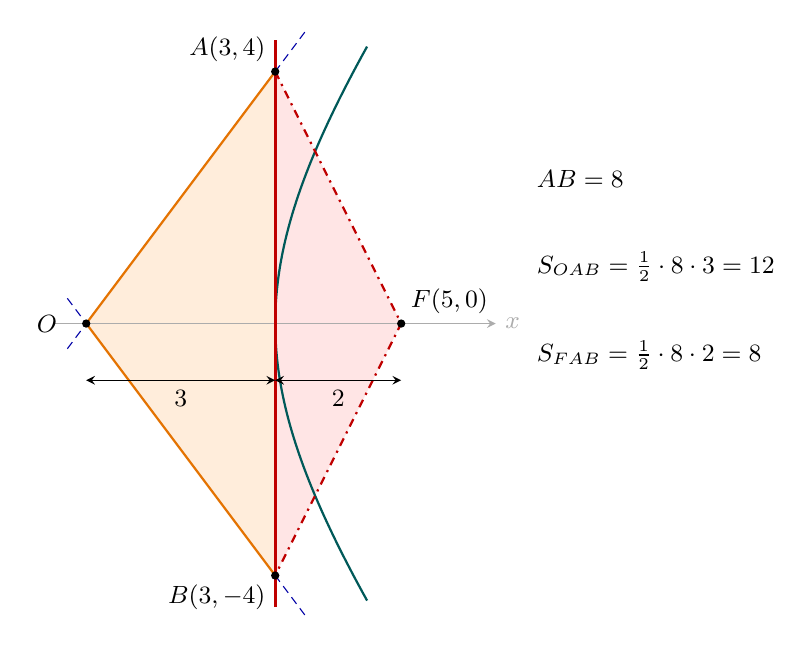
\begin{tikzpicture}[x=.8cm,y=.8cm,>=stealth,every node/.style={font=\small}]
\coordinate (O) at (0,0);\coordinate (F) at (5,0);
\coordinate (A) at (3,4);\coordinate (B) at (3,-4);
\fill[orange!14] (O)--(A)--(B)--cycle;
\fill[red!10] (F)--(A)--(B)--cycle;
\draw[gray!65,->] (-.5,0)--(6.5,0) node[right] {$x$};
\draw[blue!65!black,densely dashed] (-.3,-.4)--(3.5,4.666667);
\draw[blue!65!black,densely dashed] (-.3,.4)--(3.5,-4.666667);
\draw[teal!70!black,thick,domain=-.95:.95,samples=80,variable=\t]
 plot ({1.5*(exp(\t)+exp(-\t))},{2*(exp(\t)-exp(-\t))});
\draw[red!75!black,very thick] (3,-4.5)--(3,4.5);
\draw[orange!90!black,thick] (A)--(O)--(B);
\draw[red!75!black,thick,dash dot] (A)--(F)--(B);
\fill (O) circle(1.5pt) node[left=7pt] {$O$};
\fill (F) circle(1.5pt) node[above right] {$F(5,0)$};
\fill (A) circle(1.5pt) node[above left] {$A(3,4)$};
\fill (B) circle(1.5pt) node[below left] {$B(3,-4)$};
\draw[<->] (0,-.9)--(3,-.9) node[midway,below] {$3$};
\draw[<->] (3,-.9)--(5,-.9) node[midway,below] {$2$};
\node[anchor=west] at (7,2.3) {$AB=8$};
\node[anchor=west] at (7,.9) {$S_{OAB}=\frac12\cdot8\cdot3=12$};
\node[anchor=west] at (7,-.5) {$S_{FAB}=\frac12\cdot8\cdot2=8$};
\end{tikzpicture}

\end{center}
\begin{itemize}
\item \textbf{误认 $AB$ 或 $OA$、$OB$ 分别恒定。}
只有 $OA\cdot OB=a^2+b^2$ 恒定；两段长度通常都改变。
顶点时 $AB=2b$，一般点时 $AB$ 不必等于 $2b$。
\item \textbf{把 $OA\cdot OB$ 写成 $OA^2+OB^2$。}
一个是长度之积，一个是平方和；且都不是向量点积。
\item \textbf{忘记切点可能是顶点。} 
斜截式 $y=kx+d$ 会遗漏竖直切线 $x=\pm a$；
用标准切线式 $xx_0/a^2-yy_0/b^2=1$ 最稳妥。
\item \textbf{只用右支的正参数推出``全曲线成立''。}
切点在左支时交点横坐标可为负；面积要取绝对值。
标准切线式中的 $(u-v)(u+v)=1$ 对两支均成立。
\item \textbf{中点结论不能凭示意图宣称。}
$P$ 是 $AB$ 的中点由切线方程严格推出，绝非对任意割线成立。
\end{itemize}
\textbf{反例诊断：}面积从 $6$ 变成 $24$ 时，第一时间检查：
这条直线真的与双曲线\textbf{相切}吗？
\end{trapbox}
